\section{Optimal Control of Pitch/Travel with Feedback (LQ)}\label{sec:10.3}
\subsection{The Linear Quadratic Regulator} \label{subsec:lqr}
In this section feedback is introduced to our system by implementing a Linear Quadratic Regulator (LQR). The feedback data is obtained by subtracting the calculated optimal states from the measured states. If a deviation occurs, the controller compensates by altering the control input $u_{k}$, given by
\begin{equation}\label{eq:feedBackGain}
u_{k} = u_{k}^*-K^\top(x_{k}-x_{k}^*)
\end{equation}

\begin{figure}[H]
\includegraphics[width=1\linewidth, height=7cm]{figures/LQR_model} 
\centering
\caption{Simulink diagram of the Linear Quadratic Controller}\label{fig:figur7}
\end{figure}

The LQR is implemented in Simulink and an optimal gain matrix $K$ is found by using the MATLAB function \texttt{dlqr}, which calculates $K$ by using the infinite horizon solution $S$ of the associated discrete-time Riccati equation \cite{MathWorks}:

\begin{equation}\label{eq:gainMatrix}
K = (B^\top SB+R)^{-1}(B^\top SA)
\end{equation}

This modification leads to a change in the control hierachy, illustrated in Figure \ref{fig:figur8}.

\begin{figure}[H]
\includegraphics[width=1\linewidth, height=7cm]{figures/10_3ControlHieraky} 
\centering
\caption{Updated hiearchy with LQR}\label{fig:figur8}
\end{figure}\\

The quadratic function to be minimized by the controller is

\begin{subequations}\label{eq:10_3_linmod}
\begin{equation}\label{eq:10_3_objfunc}
J = \sum_{i=0}^{\infty} \triangle x_{i+1}^\top Q_{lqr} \triangle x_{i+1}+\triangle u_{i}^\top R_{lqr} \triangle u_{i},\quad Q_{lqr}\geq 0,\quad R_{lqr}>0
\end{equation}
\begin{equation}
\triangle x_{i+1} = A\triangle x_{i} + B\triangle u_{i} \end{equation}
\begin{equation}
\triangle x = x - x^*        
\end{equation}
\begin{equation}
\triangle u = u - u^*        
\end{equation}		
\end{subequations}

where $Q_{lqr}$ and $R_{lqr}$ are diagonal matrices that are used to penalize deviation in the states or in the feedback variable $u_{k}$.

\newpage
\subsection{Results and discussion}
The system was implemented and tested with different values of Q and R, focusing on travel. Satisfactory results were found by adding a small penalty on the input deviations, making the helicopter react faster. 

\begin{equation}
{Q_{lqr}} = \left[ {\begin{array}{*{20}{c}}
{1}&0&0&0\\
0&0&0&0\\
0&0&0&0\\
0&0&0&0
\end{array}} \right],\quad {R_{lqr}} = 0.1
\end{equation}


\begin{figure}[H]
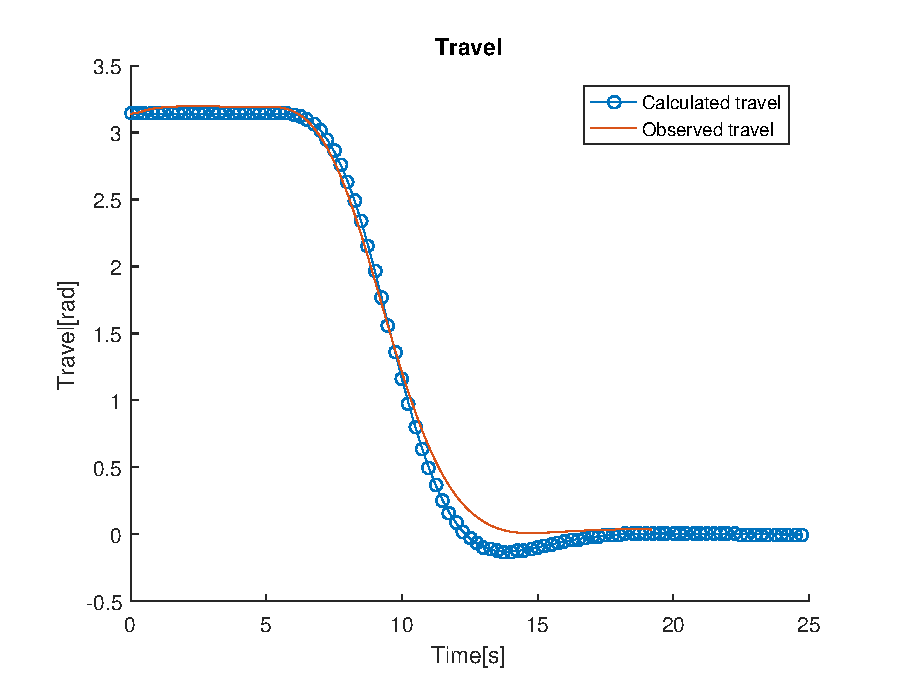
\includegraphics[scale=0.73]{data_10.3/10_3_travel_opt_and_observed} 
\centering
\caption{Observed travel ($\lambda$) compared to calculated trajectory}\label{fig:figur9}
\end{figure}

\begin{figure}[H]
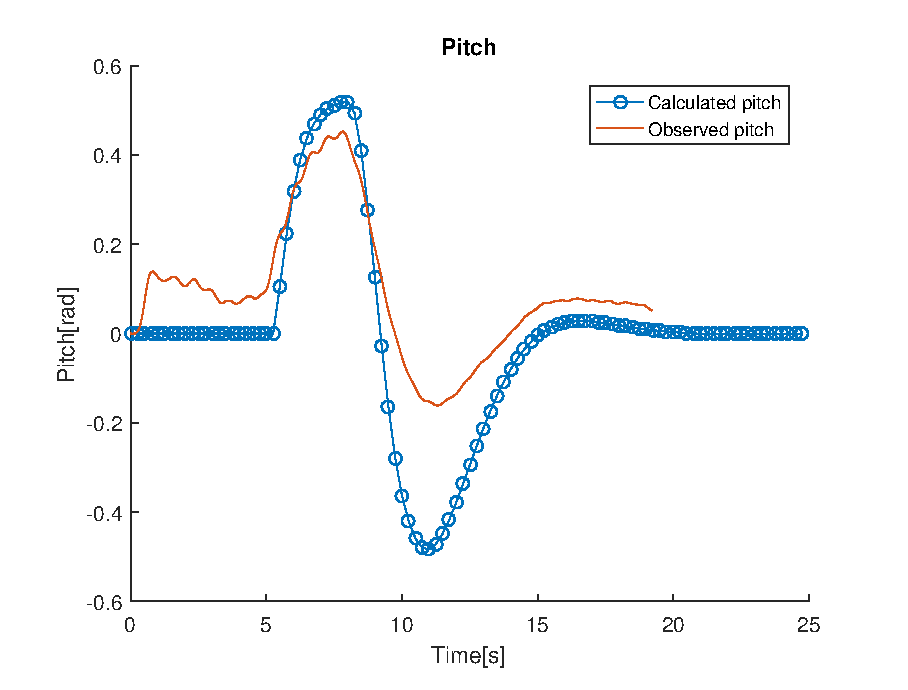
\includegraphics[scale=0.73]{data_10.3/10_3_pitch_opt_and_observed} 
\centering
\caption{Observed pitch ($p$) compared to calculated values}\label{fig:figur9}
\end{figure}

As seen from figure 11 and 12, the measured travel follows the calculated trajectory quite well, while the measured pitch has slight deviations. As seen in the case without feedback in Section \ref{sec:10.2}, the helicopter starts drifting away after it has reached its desired destination. It also starts off with a small pitch angle. This does not happen in this section, meaning that feedback can be used as a utility to compensate for disturbances and model inaccuracies. 

\subsubsection{Alternative control strategies}
Instead of using an LQ controller, Model Predictive Control (MPC) could be used. MPC would be implemented by using the current state as the initial value and solving an open-loop optimal control problem at each time step, over a specified time interval. The first control in the output sequence is then applied to the system and the process repeats itself. A disadvantage compared to the LQR case is that it costs more computationally. In addition, the performance of an MPC is highly dependent on having well tuned PID controllers in the control layer. In this lab it might be wise to retune the controllers to ensure that this is the case before implementation of an MPC. It is also important that the physical model is as accurate as possible. Given this, an MPC would most likely give better performance with better reference tracking and disturbance rejection compared to an LQR.   \cite{Foss2016} 





